\documentclass[12pt]{article}

%packages
%\usepackage{latexsym}
\usepackage{graphicx}
\usepackage{color}
\usepackage{amsmath}
\usepackage{dsfont}
\usepackage{placeins}
\usepackage{amssymb}
\usepackage{wasysym}
\usepackage{abstract}
\usepackage{hyperref}
\usepackage{etoolbox}
\usepackage{datetime}
\usepackage{xcolor}
\settimeformat{ampmtime}

%\usepackage{pstricks,pst-node,pst-tree}

%\usepackage{algpseudocode}
%\usepackage{amsthm}
%\usepackage{hyperref}
%\usepackage{mathrsfs}
%\usepackage{amsfonts}
%\usepackage{bbding}
%\usepackage{listings}
%\usepackage{appendix}
\usepackage[margin=1in]{geometry}
%\geometry{papersize={8.5in,11in},total={6.5in,9in}}
%\usepackage{cancel}
%\usepackage{algorithmic, algorithm}

\makeatletter
\def\maxwidth{ %
  \ifdim\Gin@nat@width>\linewidth
    \linewidth
  \else
    \Gin@nat@width
  \fi
}
\makeatother

\definecolor{fgcolor}{rgb}{0.345, 0.345, 0.345}
\newcommand{\hlnum}[1]{\textcolor[rgb]{0.686,0.059,0.569}{#1}}%
\newcommand{\hlstr}[1]{\textcolor[rgb]{0.192,0.494,0.8}{#1}}%
\newcommand{\hlcom}[1]{\textcolor[rgb]{0.678,0.584,0.686}{\textit{#1}}}%
\newcommand{\hlopt}[1]{\textcolor[rgb]{0,0,0}{#1}}%
\newcommand{\hlstd}[1]{\textcolor[rgb]{0.345,0.345,0.345}{#1}}%
\newcommand{\hlkwa}[1]{\textcolor[rgb]{0.161,0.373,0.58}{\textbf{#1}}}%
\newcommand{\hlkwb}[1]{\textcolor[rgb]{0.69,0.353,0.396}{#1}}%
\newcommand{\hlkwc}[1]{\textcolor[rgb]{0.333,0.667,0.333}{#1}}%
\newcommand{\hlkwd}[1]{\textcolor[rgb]{0.737,0.353,0.396}{\textbf{#1}}}%

\usepackage{framed}
\makeatletter
\newenvironment{kframe}{%
 \def\at@end@of@kframe{}%
 \ifinner\ifhmode%
  \def\at@end@of@kframe{\end{minipage}}%
  \begin{minipage}{\columnwidth}%
 \fi\fi%
 \def\FrameCommand##1{\hskip\@totalleftmargin \hskip-\fboxsep
 \colorbox{shadecolor}{##1}\hskip-\fboxsep
     % There is no \\@totalrightmargin, so:
     \hskip-\linewidth \hskip-\@totalleftmargin \hskip\columnwidth}%
 \MakeFramed {\advance\hsize-\width
   \@totalleftmargin\z@ \linewidth\hsize
   \@setminipage}}%
 {\par\unskip\endMakeFramed%
 \at@end@of@kframe}
\makeatother

\definecolor{shadecolor}{rgb}{.77, .77, .77}
\definecolor{messagecolor}{rgb}{0, 0, 0}
\definecolor{warningcolor}{rgb}{1, 0, 1}
\definecolor{errorcolor}{rgb}{1, 0, 0}
\newenvironment{knitrout}{}{} % an empty environment to be redefined in TeX

\usepackage{alltt}
\usepackage[T1]{fontenc}

\newcommand{\qu}[1]{``#1''}
\newcounter{probnum}
\setcounter{probnum}{1}

%create definition to allow local margin changes
\def\changemargin#1#2{\list{}{\rightmargin#2\leftmargin#1}\item[]}
\let\endchangemargin=\endlist 

%allow equations to span multiple pages
\allowdisplaybreaks

%define colors and color typesetting conveniences
\definecolor{gray}{rgb}{0.5,0.5,0.5}
\definecolor{black}{rgb}{0,0,0}
\definecolor{white}{rgb}{1,1,1}
\definecolor{blue}{rgb}{0.5,0.5,1}
\newcommand{\inblue}[1]{\color{blue}#1 \color{black}}
\definecolor{green}{rgb}{0.133,0.545,0.133}
\newcommand{\ingreen}[1]{\color{green}#1 \color{black}}
\definecolor{yellow}{rgb}{1,1,0}
\newcommand{\inyellow}[1]{\color{yellow}#1 \color{black}}
\definecolor{orange}{rgb}{0.9,0.649,0}
\newcommand{\inorange}[1]{\color{orange}#1 \color{black}}
\definecolor{red}{rgb}{1,0.133,0.133}
\newcommand{\inred}[1]{\color{red}#1 \color{black}}
\definecolor{purple}{rgb}{0.58,0,0.827}
\newcommand{\inpurple}[1]{\color{purple}#1 \color{black}}
\definecolor{backgcode}{rgb}{0.97,0.97,0.8}
\definecolor{Brown}{cmyk}{0,0.81,1,0.60}
\definecolor{OliveGreen}{cmyk}{0.64,0,0.95,0.40}
\definecolor{CadetBlue}{cmyk}{0.62,0.57,0.23,0}

%define new math operators
\DeclareMathOperator*{\argmax}{arg\,max~}
\DeclareMathOperator*{\argmin}{arg\,min~}
\DeclareMathOperator*{\argsup}{arg\,sup~}
\DeclareMathOperator*{\arginf}{arg\,inf~}
\DeclareMathOperator*{\convolution}{\text{\Huge{$\ast$}}}
\newcommand{\infconv}[2]{\convolution^\infty_{#1 = 1} #2}
%true functions

%%%% GENERAL SHORTCUTS

%shortcuts for pure typesetting conveniences
\newcommand{\bv}[1]{\boldsymbol{#1}}

%shortcuts for compound constants
\newcommand{\BetaDistrConst}{\dfrac{\Gamma(\alpha + \beta)}{\Gamma(\alpha)\Gamma(\beta)}}
\newcommand{\NormDistrConst}{\dfrac{1}{\sqrt{2\pi\sigma^2}}}

%shortcuts for conventional symbols
\newcommand{\tsq}{\tau^2}
\newcommand{\tsqh}{\hat{\tau}^2}
\newcommand{\sigsq}{\sigma^2}
\newcommand{\sigsqsq}{\parens{\sigma^2}^2}
\newcommand{\sigsqovern}{\dfrac{\sigsq}{n}}
\newcommand{\tausq}{\tau^2}
\newcommand{\tausqalpha}{\tau^2_\alpha}
\newcommand{\tausqbeta}{\tau^2_\beta}
\newcommand{\tausqsigma}{\tau^2_\sigma}
\newcommand{\betasq}{\beta^2}
\newcommand{\sigsqvec}{\bv{\sigma}^2}
\newcommand{\sigsqhat}{\hat{\sigma}^2}
\newcommand{\sigsqhatmlebayes}{\sigsqhat_{\text{Bayes, MLE}}}
\newcommand{\sigsqhatmle}[1]{\sigsqhat_{#1, \text{MLE}}}
\newcommand{\bSigma}{\bv{\Sigma}}
\newcommand{\bSigmainv}{\bSigma^{-1}}
\newcommand{\thetavec}{\bv{\theta}}
\newcommand{\thetahat}{\hat{\theta}}
\newcommand{\thetahatmle}{\hat{\theta}_{\mathrm{MLE}}}
\newcommand{\thetavechatmle}{\hat{\thetavec}_{\mathrm{MLE}}}
\newcommand{\muhat}{\hat{\mu}}
\newcommand{\musq}{\mu^2}
\newcommand{\muvec}{\bv{\mu}}
\newcommand{\muhatmle}{\muhat_{\text{MLE}}}
\newcommand{\lambdahat}{\hat{\lambda}}
\newcommand{\lambdahatmle}{\lambdahat_{\text{MLE}}}
\newcommand{\etavec}{\bv{\eta}}
\newcommand{\alphavec}{\bv{\alpha}}
\newcommand{\minimaxdec}{\delta^*_{\mathrm{mm}}}
\newcommand{\ybar}{\bar{y}}
\newcommand{\xbar}{\bar{x}}
\newcommand{\iid}{~{\buildrel iid \over \sim}~}
\newcommand{\inddist}{~{\buildrel ind \over \sim}~}
\newcommand{\approxdist}{~{\buildrel approx \over \sim}~}
\newcommand{\equalsindist}{~{\buildrel d \over =}~}
\newcommand{\loglik}[1]{\ell\parens{#1}}
\newcommand{\thetahatkminone}{\thetahat^{(k-1)}}
\newcommand{\thetahatkplusone}{\thetahat^{(k+1)}}
\newcommand{\thetahatk}{\thetahat^{(k)}}
\newcommand{\half}{\frac{1}{2}}
\newcommand{\third}{\frac{1}{3}}
\newcommand{\twothirds}{\frac{2}{3}}
\newcommand{\fourth}{\frac{1}{4}}
\newcommand{\fifth}{\frac{1}{5}}
\newcommand{\sixth}{\frac{1}{6}}

%shortcuts for vector and matrix notation
\newcommand{\A}{\bv{A}}
\newcommand{\At}{\A^T}
\newcommand{\Ainv}{\inverse{\A}}
\newcommand{\B}{\bv{B}}
\newcommand{\K}{\bv{K}}
\newcommand{\Kt}{\K^T}
\newcommand{\Kinv}{\inverse{K}}
\newcommand{\Kinvt}{(\Kinv)^T}
\newcommand{\M}{\bv{M}}
\newcommand{\Bt}{\B^T}
\newcommand{\Q}{\bv{Q}}
\newcommand{\Qt}{\Q^T}
\newcommand{\R}{\bv{R}}
\newcommand{\Rt}{\R^T}
\newcommand{\Z}{\bv{Z}}
\newcommand{\X}{\bv{X}}
\newcommand{\Xsub}{\X_{\text{(sub)}}}
\newcommand{\Xsubadj}{\X_{\text{(sub,adj)}}}
\newcommand{\I}{\bv{I}}
\newcommand{\Y}{\bv{Y}}
\newcommand{\sigsqI}{\sigsq\I}
\renewcommand{\P}{\bv{P}}
\newcommand{\Psub}{\P_{\text{(sub)}}}
\newcommand{\Pt}{\P^T}
\newcommand{\Pii}{P_{ii}}
\newcommand{\Pij}{P_{ij}}
\newcommand{\IminP}{(\I-\P)}
\newcommand{\Xt}{\bv{X}^T}
\newcommand{\XtX}{\Xt\X}
\newcommand{\XtXinv}{\parens{\Xt\X}^{-1}}
\newcommand{\XtXinvXt}{\XtXinv\Xt}
\newcommand{\XXtXinvXt}{\X\XtXinvXt}
\newcommand{\x}{\bv{x}}
\newcommand{\onevec}{\bv{1}}
\newcommand{\oneton}{1, \ldots, n}
\newcommand{\yoneton}{y_1, \ldots, y_n}
\newcommand{\yonetonorder}{y_{(1)}, \ldots, y_{(n)}}
\newcommand{\Yoneton}{Y_1, \ldots, Y_n}
\newcommand{\iinoneton}{i \in \braces{\oneton}}
\newcommand{\onetom}{1, \ldots, m}
\newcommand{\jinonetom}{j \in \braces{\onetom}}
\newcommand{\xoneton}{x_1, \ldots, x_n}
\newcommand{\Xoneton}{X_1, \ldots, X_n}
\newcommand{\xt}{\x^T}
\newcommand{\y}{\bv{y}}
\newcommand{\yt}{\y^T}
\renewcommand{\c}{\bv{c}}
\newcommand{\ct}{\c^T}
\newcommand{\tstar}{\bv{t}^*}
\renewcommand{\u}{\bv{u}}
\renewcommand{\v}{\bv{v}}
\renewcommand{\a}{\bv{a}}
\newcommand{\s}{\bv{s}}
\newcommand{\yadj}{\y_{\text{(adj)}}}
\newcommand{\xjadj}{\x_{j\text{(adj)}}}
\newcommand{\xjadjM}{\x_{j \perp M}}
\newcommand{\yhat}{\hat{\y}}
\newcommand{\yhatsub}{\yhat_{\text{(sub)}}}
\newcommand{\yhatstar}{\yhat^*}
\newcommand{\yhatstarnew}{\yhatstar_{\text{new}}}
\newcommand{\z}{\bv{z}}
\newcommand{\zt}{\z^T}
\newcommand{\bb}{\bv{b}}
\newcommand{\bbt}{\bb^T}
\newcommand{\bbeta}{\bv{\beta}}
\newcommand{\beps}{\bv{\epsilon}}
\newcommand{\bepst}{\beps^T}
\newcommand{\e}{\bv{e}}
\newcommand{\Mofy}{\M(\y)}
\newcommand{\KofAlpha}{K(\alpha)}
\newcommand{\ellset}{\mathcal{L}}
\newcommand{\oneminalph}{1-\alpha}
\newcommand{\SSE}{\text{SSE}}
\newcommand{\SSEsub}{\text{SSE}_{\text{(sub)}}}
\newcommand{\MSE}{\text{MSE}}
\newcommand{\RMSE}{\text{RMSE}}
\newcommand{\SSR}{\text{SSR}}
\newcommand{\SST}{\text{SST}}
\newcommand{\JSest}{\delta_{\text{JS}}(\x)}
\newcommand{\Bayesest}{\delta_{\text{Bayes}}(\x)}
\newcommand{\EmpBayesest}{\delta_{\text{EmpBayes}}(\x)}
\newcommand{\BLUPest}{\delta_{\text{BLUP}}}
\newcommand{\MLEest}[1]{\hat{#1}_{\text{MLE}}}

%shortcuts for Linear Algebra stuff (i.e. vectors and matrices)
\newcommand{\twovec}[2]{\bracks{\begin{array}{c} #1 \\ #2 \end{array}}}
\newcommand{\threevec}[3]{\bracks{\begin{array}{c} #1 \\ #2 \\ #3 \end{array}}}
\newcommand{\fivevec}[5]{\bracks{\begin{array}{c} #1 \\ #2 \\ #3 \\ #4 \\ #5 \end{array}}}
\newcommand{\twobytwomat}[4]{\bracks{\begin{array}{cc} #1 & #2 \\ #3 & #4 \end{array}}}
\newcommand{\threebytwomat}[6]{\bracks{\begin{array}{cc} #1 & #2 \\ #3 & #4 \\ #5 & #6 \end{array}}}

%shortcuts for conventional compound symbols
\newcommand{\thetainthetas}{\theta \in \Theta}
\newcommand{\reals}{\mathbb{R}}
\newcommand{\complexes}{\mathbb{C}}
\newcommand{\rationals}{\mathbb{Q}}
\newcommand{\integers}{\mathbb{Z}}
\newcommand{\naturals}{\mathbb{N}}
\newcommand{\forallninN}{~~\forall n \in \naturals}
\newcommand{\forallxinN}[1]{~~\forall #1 \in \reals}
\newcommand{\matrixdims}[2]{\in \reals^{\,#1 \times #2}}
\newcommand{\inRn}[1]{\in \reals^{\,#1}}
\newcommand{\mathimplies}{\quad\Rightarrow\quad}
\newcommand{\mathlogicequiv}{\quad\Leftrightarrow\quad}
\newcommand{\eqncomment}[1]{\quad \text{(#1)}}
\newcommand{\limitn}{\lim_{n \rightarrow \infty}}
\newcommand{\limitN}{\lim_{N \rightarrow \infty}}
\newcommand{\limitd}{\lim_{d \rightarrow \infty}}
\newcommand{\limitt}{\lim_{t \rightarrow \infty}}
\newcommand{\limitsupn}{\limsup_{n \rightarrow \infty}~}
\newcommand{\limitinfn}{\liminf_{n \rightarrow \infty}~}
\newcommand{\limitk}{\lim_{k \rightarrow \infty}}
\newcommand{\limsupn}{\limsup_{n \rightarrow \infty}}
\newcommand{\limsupk}{\limsup_{k \rightarrow \infty}}
\newcommand{\floor}[1]{\left\lfloor #1 \right\rfloor}
\newcommand{\ceil}[1]{\left\lceil #1 \right\rceil}

%shortcuts for environments
\newcommand{\beqn}{\vspace{-0.25cm}\begin{eqnarray*}}
\newcommand{\eeqn}{\end{eqnarray*}}
\newcommand{\bneqn}{\vspace{-0.25cm}\begin{eqnarray}}
\newcommand{\eneqn}{\end{eqnarray}}

%shortcuts for mini environments
\newcommand{\parens}[1]{\left(#1\right)}
\newcommand{\squared}[1]{\parens{#1}^2}
\newcommand{\tothepow}[2]{\parens{#1}^{#2}}
\newcommand{\prob}[1]{\mathbb{P}\parens{#1}}
\newcommand{\cprob}[2]{\prob{#1~|~#2}}
\newcommand{\littleo}[1]{o\parens{#1}}
\newcommand{\bigo}[1]{O\parens{#1}}
\newcommand{\Lp}[1]{\mathbb{L}^{#1}}
\renewcommand{\arcsin}[1]{\text{arcsin}\parens{#1}}
\newcommand{\prodonen}[2]{\bracks{\prod_{#1=1}^n #2}}
\newcommand{\mysum}[4]{\sum_{#1=#2}^{#3} #4}
\newcommand{\sumonen}[2]{\sum_{#1=1}^n #2}
\newcommand{\infsum}[2]{\sum_{#1=1}^\infty #2}
\newcommand{\infprod}[2]{\prod_{#1=1}^\infty #2}
\newcommand{\infunion}[2]{\bigcup_{#1=1}^\infty #2}
\newcommand{\infinter}[2]{\bigcap_{#1=1}^\infty #2}
\newcommand{\infintegral}[2]{\int^\infty_{-\infty} #2 ~\text{d}#1}
\newcommand{\supthetas}[1]{\sup_{\thetainthetas}\braces{#1}}
\newcommand{\bracks}[1]{\left[#1\right]}
\newcommand{\braces}[1]{\left\{#1\right\}}
\newcommand{\set}[1]{\left\{#1\right\}}
\newcommand{\abss}[1]{\left|#1\right|}
\newcommand{\norm}[1]{\left|\left|#1\right|\right|}
\newcommand{\normsq}[1]{\norm{#1}^2}
\newcommand{\inverse}[1]{\parens{#1}^{-1}}
\newcommand{\rowof}[2]{\parens{#1}_{#2\cdot}}

%shortcuts for functionals
\newcommand{\realcomp}[1]{\text{Re}\bracks{#1}}
\newcommand{\imagcomp}[1]{\text{Im}\bracks{#1}}
\newcommand{\range}[1]{\text{range}\bracks{#1}}
\newcommand{\colsp}[1]{\text{colsp}\bracks{#1}}
\newcommand{\rowsp}[1]{\text{rowsp}\bracks{#1}}
\newcommand{\tr}[1]{\text{tr}\bracks{#1}}
\newcommand{\rank}[1]{\text{rank}\bracks{#1}}
\newcommand{\proj}[2]{\text{Proj}_{#1}\bracks{#2}}
\newcommand{\projcolspX}[1]{\text{Proj}_{\colsp{\X}}\bracks{#1}}
\newcommand{\median}[1]{\text{median}\bracks{#1}}
\newcommand{\mean}[1]{\text{mean}\bracks{#1}}
\newcommand{\dime}[1]{\text{dim}\bracks{#1}}
\renewcommand{\det}[1]{\text{det}\bracks{#1}}
\newcommand{\expe}[1]{\mathbb{E}\bracks{#1}}
\newcommand{\expeabs}[1]{\expe{\abss{#1}}}
\newcommand{\expesub}[2]{\mathbb{E}_{#1}\bracks{#2}}
\newcommand{\indic}[1]{\mathds{1}_{#1}}
\newcommand{\var}[1]{\text{Var}\bracks{#1}}
\newcommand{\cov}[2]{\text{Cov}\bracks{#1, #2}}
\newcommand{\corr}[2]{\text{Corr}\bracks{#1, #2}}
\newcommand{\se}[1]{\text{SE}\bracks{#1}}
\newcommand{\seest}[1]{\hat{\text{SE}}\bracks{#1}}
\newcommand{\bias}[1]{\text{Bias}\bracks{#1}}
\newcommand{\partialop}[2]{\dfrac{\partial}{\partial #1}\bracks{#2}}
\newcommand{\secpartialop}[2]{\dfrac{\partial^2}{\partial #1^2}\bracks{#2}}
\newcommand{\mixpartialop}[3]{\dfrac{\partial^2}{\partial #1 \partial #2}\bracks{#3}}

%shortcuts for functions
\renewcommand{\exp}[1]{\mathrm{exp}\parens{#1}}
\renewcommand{\cos}[1]{\text{cos}\parens{#1}}
\renewcommand{\sin}[1]{\text{sin}\parens{#1}}
\newcommand{\sign}[1]{\text{sign}\parens{#1}}
\newcommand{\are}[1]{\mathrm{ARE}\parens{#1}}
\newcommand{\natlog}[1]{\ln\parens{#1}}
\newcommand{\oneover}[1]{\frac{1}{#1}}
\newcommand{\overtwo}[1]{\frac{#1}{2}}
\newcommand{\overn}[1]{\frac{#1}{n}}
\newcommand{\oneoversqrt}[1]{\oneover{\sqrt{#1}}}
\newcommand{\sqd}[1]{\parens{#1}^2}
\newcommand{\loss}[1]{\ell\parens{\theta, #1}}
\newcommand{\losstwo}[2]{\ell\parens{#1, #2}}
\newcommand{\cf}{\phi(t)}

%English language specific shortcuts
\newcommand{\ie}{\textit{i.e.} }
\newcommand{\AKA}{\textit{AKA} }
\renewcommand{\iff}{\textit{iff}}
\newcommand{\eg}{\textit{e.g.} }
\newcommand{\st}{\textit{s.t.} }
\newcommand{\wrt}{\textit{w.r.t.} }
\newcommand{\mathst}{~~\text{\st}~~}
\newcommand{\mathand}{~~\text{and}~~}
\newcommand{\ala}{\textit{a la} }
\newcommand{\ppp}{posterior predictive p-value}
\newcommand{\dd}{dataset-to-dataset}

%shortcuts for distribution titles
\newcommand{\logistic}[2]{\mathrm{Logistic}\parens{#1,\,#2}}
\newcommand{\bernoulli}[1]{\mathrm{Bernoulli}\parens{#1}}
\newcommand{\betanot}[2]{\mathrm{Beta}\parens{#1,\,#2}}
\newcommand{\stdbetanot}{\betanot{\alpha}{\beta}}
\newcommand{\multnormnot}[3]{\mathcal{N}_{#1}\parens{#2,\,#3}}
\newcommand{\normnot}[2]{\mathcal{N}\parens{#1,\,#2}}
\newcommand{\classicnormnot}{\normnot{\mu}{\sigsq}}
\newcommand{\stdnormnot}{\normnot{0}{1}}
\newcommand{\uniform}[2]{\mathrm{U}\parens{#1,\,#2}}
\newcommand{\stduniform}{\uniform{0}{1}}
\newcommand{\exponential}[1]{\mathrm{Exp}\parens{#1}}
\newcommand{\gammadist}[2]{\mathrm{Gamma}\parens{#1, #2}}
\newcommand{\poisson}[1]{\mathrm{Poisson}\parens{#1}}
\newcommand{\binomial}[2]{\mathrm{Binomial}\parens{#1,\,#2}}
\newcommand{\rayleigh}[1]{\mathrm{Rayleigh}\parens{#1}}
\newcommand{\multinomial}[2]{\mathrm{Multinomial}\parens{#1,\,#2}}
\newcommand{\gammanot}[2]{\mathrm{Gamma}\parens{#1,\,#2}}
\newcommand{\cauchynot}[2]{\text{Cauchy}\parens{#1,\,#2}}
\newcommand{\invchisqnot}[1]{\text{Inv}\chisq{#1}}
\newcommand{\invscaledchisqnot}[2]{\text{ScaledInv}\ncchisq{#1}{#2}}
\newcommand{\invgammanot}[2]{\text{InvGamma}\parens{#1,\,#2}}
\newcommand{\chisq}[1]{\chi^2_{#1}}
\newcommand{\ncchisq}[2]{\chi^2_{#1}\parens{#2}}
\newcommand{\ncF}[3]{F_{#1,#2}\parens{#3}}

%shortcuts for PDF's of common distributions
\newcommand{\logisticpdf}[3]{\oneover{#3}\dfrac{\exp{-\dfrac{#1 - #2}{#3}}}{\parens{1+\exp{-\dfrac{#1 - #2}{#3}}}^2}}
\newcommand{\betapdf}[3]{\dfrac{\Gamma(#2 + #3)}{\Gamma(#2)\Gamma(#3)}#1^{#2-1} (1-#1)^{#3-1}}
\newcommand{\normpdf}[3]{\frac{1}{\sqrt{2\pi#3}}\exp{-\frac{1}{2#3}(#1 - #2)^2}}
\newcommand{\normpdfvarone}[2]{\dfrac{1}{\sqrt{2\pi}}e^{-\half(#1 - #2)^2}}
\newcommand{\chisqpdf}[2]{\dfrac{1}{2^{#2/2}\Gamma(#2/2)}\; {#1}^{#2/2-1} e^{-#1/2}}
\newcommand{\invchisqpdf}[2]{\dfrac{2^{-\overtwo{#1}}}{\Gamma(#2/2)}\,{#1}^{-\overtwo{#2}-1}  e^{-\oneover{2 #1}}}
\newcommand{\exponentialpdf}[2]{#2\exp{-#2#1}}
\newcommand{\poissonpdf}[2]{\dfrac{e^{-#1} #1^{#2}}{#2!}}
\newcommand{\binomialpdf}[3]{\binom{#2}{#1}#3^{#1}(1-#3)^{#2-#1}}
\newcommand{\rayleighpdf}[2]{\dfrac{#1}{#2^2}\exp{-\dfrac{#1^2}{2 #2^2}}}
\newcommand{\gammapdf}[3]{\dfrac{#3^#2}{\Gamma\parens{#2}}#1^{#2-1}\exp{-#3 #1}}
\newcommand{\cauchypdf}[3]{\oneover{\pi} \dfrac{#3}{\parens{#1-#2}^2 + #3^2}}
\newcommand{\Gammaf}[1]{\Gamma\parens{#1}}

%shortcuts for miscellaneous typesetting conveniences
\newcommand{\notesref}[1]{\marginpar{\color{gray}\tt #1\color{black}}}

%%%% DOMAIN-SPECIFIC SHORTCUTS

%Real analysis related shortcuts
\newcommand{\zeroonecl}{\bracks{0,1}}
\newcommand{\forallepsgrzero}{\forall \epsilon > 0~~}
\newcommand{\lessthaneps}{< \epsilon}
\newcommand{\fraccomp}[1]{\text{frac}\bracks{#1}}

%Bayesian related shortcuts
\newcommand{\yrep}{y^{\text{rep}}}
\newcommand{\yrepisq}{(\yrep_i)^2}
\newcommand{\yrepvec}{\bv{y}^{\text{rep}}}


%Probability shortcuts
\newcommand{\SigField}{\mathcal{F}}
\newcommand{\ProbMap}{\mathcal{P}}
\newcommand{\probtrinity}{\parens{\Omega, \SigField, \ProbMap}}
\newcommand{\convp}{~{\buildrel p \over \rightarrow}~}
\newcommand{\convLp}[1]{~{\buildrel \Lp{#1} \over \rightarrow}~}
\newcommand{\nconvp}{~{\buildrel p \over \nrightarrow}~}
\newcommand{\convae}{~{\buildrel a.e. \over \longrightarrow}~}
\newcommand{\convau}{~{\buildrel a.u. \over \longrightarrow}~}
\newcommand{\nconvau}{~{\buildrel a.u. \over \nrightarrow}~}
\newcommand{\nconvae}{~{\buildrel a.e. \over \nrightarrow}~}
\newcommand{\convd}{~{\buildrel \mathcal{D} \over \rightarrow}~}
\newcommand{\nconvd}{~{\buildrel \mathcal{D} \over \nrightarrow}~}
\newcommand{\withprob}{~~\text{w.p.}~~}
\newcommand{\io}{~~\text{i.o.}}

\newcommand{\Acl}{\bar{A}}
\newcommand{\ENcl}{\bar{E}_N}
\newcommand{\diam}[1]{\text{diam}\parens{#1}}

\newcommand{\taua}{\tau_a}

\newcommand{\myint}[4]{\int_{#2}^{#3} #4 \,\text{d}#1}
\newcommand{\laplacet}[1]{\mathscr{L}\bracks{#1}}
\newcommand{\laplaceinvt}[1]{\mathscr{L}^{-1}\bracks{#1}}
\renewcommand{\min}[1]{\text{min}\braces{#1}}

\newcommand{\Vbar}[1]{\bar{V}\parens{#1}}
\newcommand{\expnegrtau}{\exp{-r\tau}}

%%% problem typesetting
\newcommand{\problem}{\noindent \colorbox{black}{{\color{yellow} \large{\textsf{\textbf{Problem \arabic{probnum}}}}~}} \addtocounter{probnum}{1} \vspace{0.2cm} \\ }

\newcommand{\easysubproblem}{\ingreen{\item}}
\newcommand{\intermediatesubproblem}{\inorange{\item}}
\newcommand{\hardsubproblem}{\inred{\item}}
\newcommand{\extracreditsubproblem}{\inpurple{\item} [E.C.] }
\renewcommand{\labelenumi}{(\alph{enumi})}




\title{Math 241 Fall 2014-2015 \\ Final Examination}
\author{Professor Adam Kapelner}

\date{December 18, 2014}

\begin{document}
\maketitle

\noindent Full Name \line(1,0){270} ~~~ Section (A or B)~ \line(1,0){30}

\thispagestyle{empty}

\section*{Code of Academic Integrity}

\footnotesize
Since the college is an academic community, its fundamental purpose is the pursuit of knowledge. Essential to the success of this educational mission is a commitment to the principles of academic integrity. Every member of the college community is responsible for upholding the highest standards of honesty at all times. Students, as members of the community, are also responsible for adhering to the principles and spirit of the following Code of Academic Integrity.

Activities that have the effect or intention of interfering with education, pursuit of knowledge, or fair evaluation of a student's performance are prohibited. Examples of such activities include but are not limited to the following definition:

\paragraph{Cheating} Using or attempting to use unauthorized assistance, material, or study aids in examinations or other academic work or preventing, or attempting to prevent, another from using authorized assistance, material, or study aids. Example: using an unauthorized cheat sheet in a quiz or exam, altering a graded exam and resubmitting it for a better grade, etc.
\\

\noindent I acknowledge and agree to uphold this Code of Academic Integrity. \\

\begin{center}
\line(1,0){250} ~~~ \line(1,0){100}\\
~~~~~~~~~~~~~~~~~~~~~signature~~~~~~~~~~~~~~~~~~~~~~~~~~~~~~~~~~~~~~~~~~~~~ date
\end{center}

\normalsize

\section*{Instructions}

This exam is 120 minutes and closed-book. You are allowed three pages (front and back) of a \qu{cheat sheet.} You may use a graphing calculator of your choice. Please read the questions carefully. If I say \qu{compute,} this means the solution will be a number. I also advise you to use pencil.\\

\noindent The exam is 100 points total. Partial credit will be granted for incomplete answers on most of the questions. I advise you to skip problems marked \qu{[Extra Credit]} until you have finished the other questions on the exam \fbox{Box} in your final answers. Good luck!

\pagebreak

\problem In this problem, we will investigate mock situations involving waiting for the Q64 bus.

\begin{figure}[h]
\begin{center}
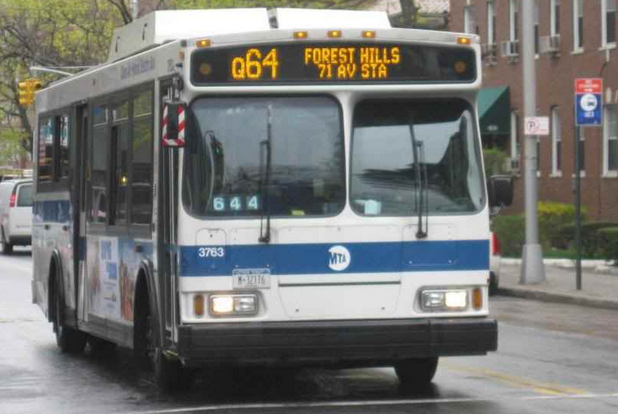
\includegraphics[width=3in]{q64.png}
\end{center}
\end{figure}


\benum
\subquestionwithpoints{4} Let's say the Q64 is scheduled during rush hour to come every 8 min. Assume the bus really does keep to this schedule. You show up at the bus stop during rush hour at a random time. What is the probability you wait more than 2min for the next Q64 bus? \spc{5}

\subquestionwithpoints{4} Let's say the time when the next Q64 comes can be modeled as $T \sim \exponential{\lambda = 0.125}$ where the support of the r.v. is measured in minutes. What is the probability you wait more than 2min for the next Q64 bus? \spc{5}

\subquestionwithpoints{3} Let's say the time when the next Q64 comes can be modeled as $T \sim \exponential{\lambda = 0.125}$ where the support is measured in minutes. You've been sitting at the bus stop and have already waited two minutes. What is the probability given that you've been waiting that you wait more than \textit{another} 2min for the next Q64 bus? \spc{5}

\eenum


\problem In this problem, we will investigate moment generating functions (mgf's) and the Central Limit Theorem.

\begin{figure}[h]
\begin{center}
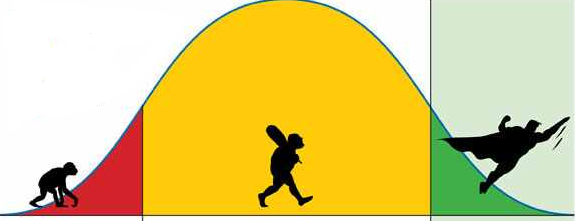
\includegraphics[width=3in]{clt.png}
\end{center}
\end{figure}


\benum

\subquestionwithpoints{4} Let $X \sim \bernoulli{\half}$. Show that $M_X(t)$, the mgf of $X$ is $\half(1+e^t)$.\spc{3}

\subquestionwithpoints{4} Set up an infinite sum that if solved would provide the mgf for $X$, a Poisson r.v. with parameter $\lambda$.  Do not attempt to solve or simplify! \spc{5}

%\subquestionwithpoints{3} Set up an improper integral that if solved would provide the mgf for an Exponential r.v. with parameter $\lambda$. Do not attempt to solve or simplify! \spc{3}

\subquestionwithpoints{4} If $X \sim \text{Erlang}(k, \lambda)$, which is the continuous analogue of the negative binomial distribution, then the PDF of $X$ is $f(x) = \frac{\lambda^k x^{k-1} e^{-\lambda k}}{(k-1)!}$ and its mgf is $M_X(t) = (1 - t/\lambda)^{-k}$. Show that $\expe{X} = k/\lambda$ using any method you wish. If you cannot solve all the way, describe the method you would use to solve for partial credit. Hint: be careful with the negative sign.\spc{6}

\subquestionwithpoints{4} If $Z_1, Z_2 \iid \stdnormnot$ what is the mgf of $
\oneoversqrt{2}Z_1 + \oneoversqrt{2}Z_2$? Hint: the mgf for the standard normal is $M_Z(t) = e^{t^2/2}$.\spc{6}

%\subquestionwithpoints{3} If $X \sim \normnot{\mu}{\sigsq}$ then $M_X(t) =e^{\mu t + \overtwo{\sigsq t^2}}$. Use this fact and the answer from the previous problem to demonstrate that $\se{Z_1 + Z_2} = \sqrt{2}$. \spc{3}


\subquestionwithpoints{3} If $X_1, \ldots, X_n \iid$ with some unknown distribution that has finite mean and variance, what is the distribution of the following quantity as $n$ gets large? Write your answer to the right of the \qu{distributed as} symbol. The brand name notation with the correct parameters clearly marked or the PDF is valid. No other answer is valid.

\beqn
\frac{\Xbar - \mu}{\frac{\sigma}{\sqrt{n}}} \sim \quad\quad\quad\quad\quad\quad\quad\quad\quad\quad\quad\quad
\eeqn \spc{0}

\subquestionwithpoints{3} We are interested in using confidence intervals and hypothesis testing for a sample and we have an idea of the distribution of the underlying r.v. which is sampled $\iid$ from a well-specified population. The following image is the result of some simulations. Below what \textit{minimum} sample size what you not trust the validity of confidence intervals and hypothesis tests? Write $n < $ something below the image.

\begin{changemargin}{-0.6in}{0in}
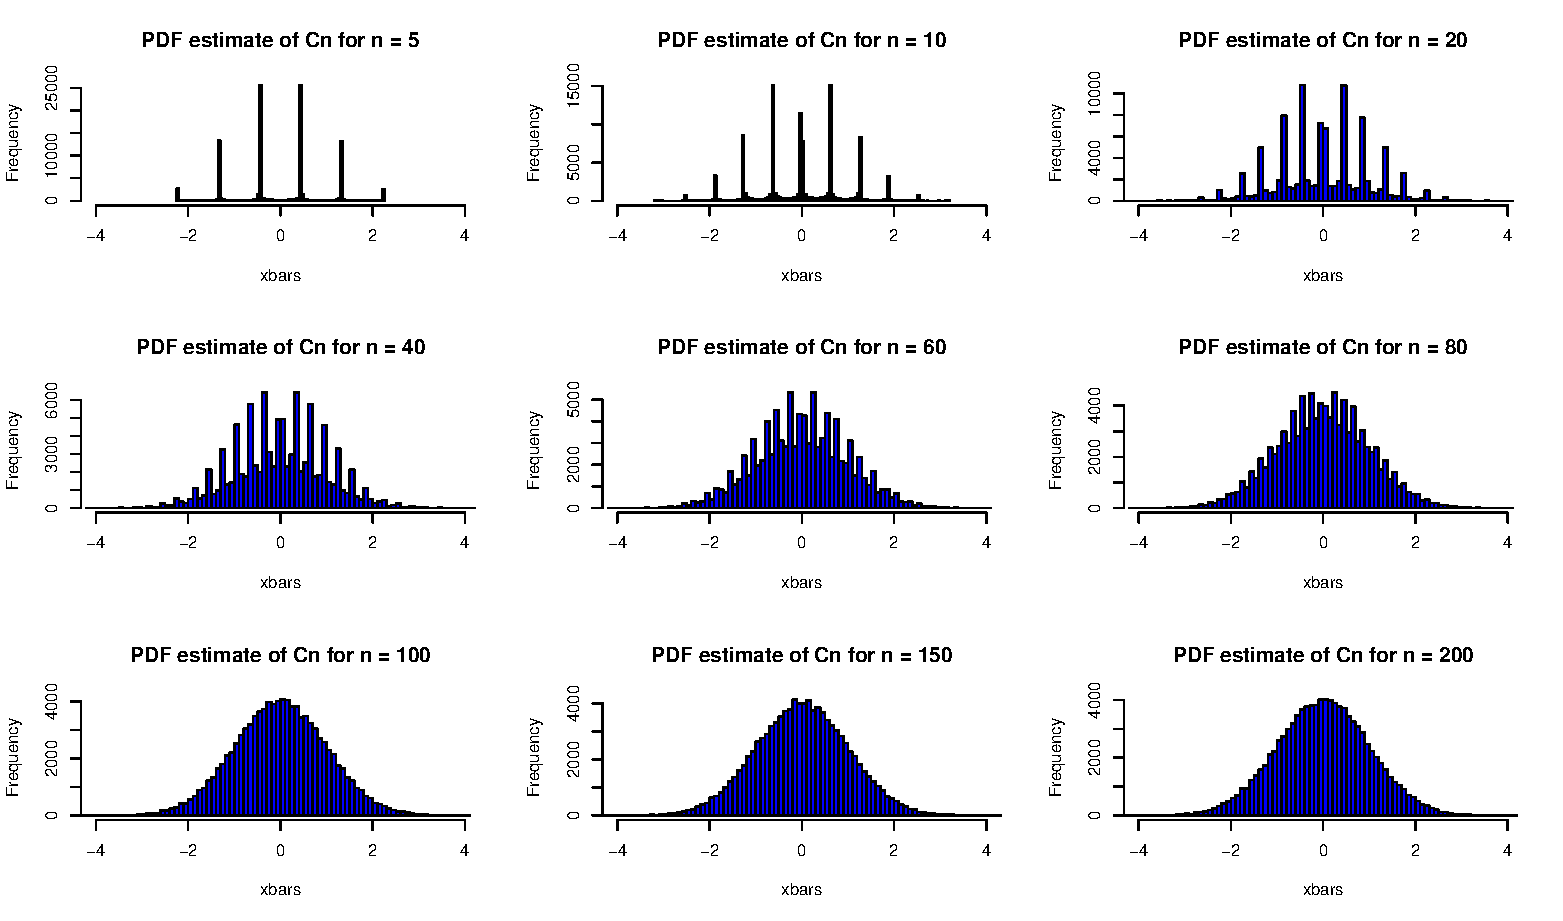
\includegraphics[width=7in]{clt.pdf}
\end{changemargin}


\eenum
\pagebreak

\problem In this problem, we will be investigating a call center. Callers call in and are helped by a customer service representative and then answer a survey later if they're satisfied or not: \qu{yes} or \qu{no.} Note that the vast majority of callers do not bother with the survey and just hang up, thus we don't know if they were satisfied or not. Assume the satisfaction outcome of all calls are $\iid$ Bernoulli r.v.'s.

\begin{figure}[h]
\begin{center}

\includegraphics[width=3in]{callcenter.jpg}
\end{center}
\end{figure}

\benum

\subquestionwithpoints{2} The company is interested in investigating George, one of the customer service representatives, on the basis of surveyed customer satisfaction. They look at a random sample of 200 of George's calls and find that 168 are satisfied. Calculate $\phat$ to two decimal places. \spc{3}

\subquestionwithpoints{5} Provide a 95\% confidence interval for the true proportion of customers satisfied by George's phone call on the post-call survey.  Use correct notation for the CI with both subscripts clearly notated. Compute explicitly and round to 3 decimal places.\spc{9}

\subquestionwithpoints{3} Employ one of the two correct interpretations of confidence intervals we discussed in class to interpret this interval appropriately \textit{in English}. Do not write two interpretations, only one of the two interpretations. \spc{3}

\subquestionwithpoints{2} What can you NOT say about this interval that you may really want to say? Answer \textit{in English}. \spc{3}

\subquestionwithpoints{2} Does this also provide 95\% coverage for the true proportion of \textit{all}  callers who satisfied with George's phone assistance? Explain why or why not. Yes or no without explanation will not receive credit.\spc{4}

\subquestionwithpoints{2} The company is aiming for 90\% customer satisfaction (as measured by the survey). If the customers are satisfied less than that proportion of the time, they will be unhappy. If they are satisfied more than 90\% of the time, then representatives are probably spending too much time with each customer which will mean increased expenditure for the company. So having customer satisfaction\textit{ too low} is bad and having customer satisfaction \textit{too high }is also bad albeit for different reasons. Write the null hypothesis and alternative hypothesis clearly below. \spc{3}

\subquestionwithpoints{5} For a sample size of $n=200$, what is the acceptance region at $\alpha = 5\%$? Your answer must be in set notation. Compute explicitly and round to three decimals. \spc{3}

\subquestionwithpoints{3} Set your probability of Type I error to be 5\%. Then, using the $\phat$ (the result of the experiment) you computed in (a), run a hypothesis test using the hypotheses you provided in (f) and the acceptance region you computed in (g) and finally interpret the result \textit{in English}. \spc{3}

\subquestionwithpoints{2} [Extra Credit] Regardless of your answer to (g), the company has a policy of firing those people who do not have 90\% customer satisfaction over their phone calls. What would a type II error be from the company's perspective? Answer \textit{in English}. \spc{3}

\subquestionwithpoints{4} [Extra Credit] The company now wants to test against $H_a : p = 0.7$ to find representatives who are not satisfying the customers. How much more likely is George to belong to the $H_0$ distribution relative to the $H_a$ distribution? Partial credit given. Do not attempt until you have finished the exam.  \spc{5}

\subquestionwithpoints{5} [Extra Credit] At $\alpha=5\%$, find the probability of a Type II error given $H_a : p = 0.7$. Partial credit given. Do not attempt until you have finished the exam. \spc{7}

\eenum


\problem In the standard American \qu{pick up sticks} game, there are 30 sticks --- 1 black, 7 red, 7 blue, 8 green and 7 yellow. The sticks are shuffled at random and allowed to drop on the floor in a messy pile strewn in random directions with random overlaps such as seen below:

\begin{figure}[h]
\begin{center}
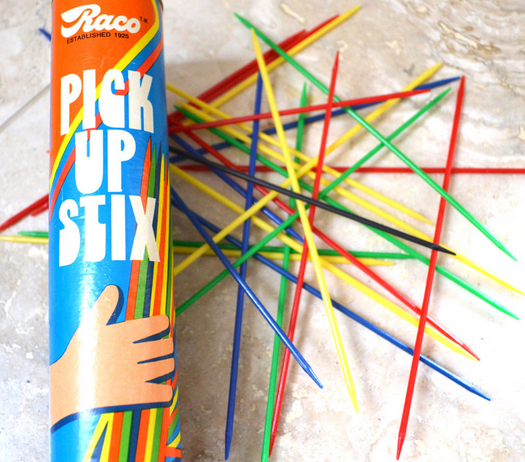
\includegraphics[width=3in]{pickup.png}
\end{center}
\end{figure}

Gameplay proceeds as follows. A player attempts to pick up a stick out of the pile without allowing any other stick to move. If they remove a stick without moving any other sticks, they collect that stick and score points and then they go again. Points are as follows: 25 points for black, 10 points for red, 5 points for blue, 2 points for green and one point for yellow. Number of sticks and points is summed up in Table~\ref{tab:pickup}.

\begin{table}[ht]
\centering
\begin{tabular}{c|cc}
Stick color & Number of sticks & Point value \\ \hline
Black & 1 & 25 \\
Red & 7 & 10 \\
Blue & 7 & 5 \\
Green & 8 & 2 \\
Yellow & 7 & 1 \\ \hline
Totals: & 30 & 153
\end{tabular}
\caption{Pick up Sticks game information}
\label{tab:pickup}
\end{table}

\benum

%\subquestionwithpoints{3} Assume a new random shuffle where the sticks allowed to drop onto a pile where every stick is on top of another stick in a specific order. What is the probability that the black stick is on top with no other sticks above it? \spc{3}

\subquestionwithpoints{2} Assume a new random shuffle. I successfully remove the top three sticks off the pile. What is the probability of (in those three sticks) getting the black stick, a red stick and a blue stick \textit{in that order}? Do \textit{not} compute explicitly. \spc{3}

%\subquestionwithpoints{3} Assume a new random shuffle. I successfully remove the top three sticks off the pile. What is the probability of (in those three sticks) having the black stick, a red stick and a blue stick \textit{in any order}? \spc{3}

\subquestionwithpoints{5} Assume a new random shuffle. At the end of the game, I have 15 sticks. What is the probability I have 3 red, 3 blue, 5 green and 4 yellow \textit{in any order}? Do \textit{not} compute explicitly.  \spc{5}

\subquestionwithpoints{2} Assume a new random shuffle. At the end of the game, I have 15 sticks. Create a r.v. that models the number of red sticks I have out of my 15 collected sticks. You should write $X \sim$ something below and write the name of the r.v. and clearly indicate the parameter(s) in this r.v. You do not have to write the PMF/PDF of this r.v. \spc{3}

%\subquestionwithpoints{3} Find the probability I wind up with 5 red sticks out of my final 15 sticks. Compute explicitly. \spc{3}

\subquestionwithpoints{2} Assume a new random shuffle. Assume the probability of me having a stick at the end of the game is 0.5 regardless of its color. Create a r.v. that models 1 if I have the black stick and 0 if I do not have the black stick. You should write $X \sim$ something below and write the name of the r.v. and clearly indicate the parameter(s) in this r.v. \spc{2}


\subquestionwithpoints{2} Assume a new random shuffle. Assume the probability of me having a stick at the end of the game is 0.5 regardless of its color. Create a r.v. that models the number of sticks I have at the end of the game regardless of their color. You should write $X \sim$ something below and write the name of the r.v. and clearly indicate the parameter(s) in this r.v. \spc{2}

\subquestionwithpoints{2} Assume a new random shuffle. Assume the probability of me having a stick at the end of the game is 0.5 regardless of its color. Find the probability I wind up with 15 sticks at the end of the game. Do \textit{not} compute explicitly but the number must be computable (no $\infty$'s allowed).  \spc{3}

\subquestionwithpoints{3} Assume a new random shuffle. Assume the probability of me having a stick at the end of the game is 0.5 regardless of its color. Find the probability I wind up with 20 or more sticks at the end of the game. Do \textit{not} compute explicitly but the number must be computable (no $\infty$'s allowed). \spc{3}

\subquestionwithpoints{4} Assume a new random shuffle. Assume the probability of me having a stick at the end of the game is 0.5 regardless of its color. Find the expected number of points I have from green sticks only. That is if you add up my score, this is the component of the score from my green sticks. \spc{3}

\subquestionwithpoints{5} [Extra Credit] Assume a new random shuffle. Assume the probability of me having a stick at the end of the game is 0.5 regardless of its color. Find the expected number of points I have at the end of the game. You can get partial credit on this extra credit.  \spc{7}

\subquestionwithpoints{2} Me and the other player are both really good at pick up sticks but it is still a difficult game. Each time we go to take a stick off, we have probability 20\% that we successfully remove the stick without jiggling another stick. What is the probability we remove three sticks successfully in three turns? Hint: you do not need to consider the fact that there are two players here. Imagine there is just one player playing against himself. \spc{3}

\subquestionwithpoints{3} Assuming we have probability 20\% that we successfully remove a stick without jiggling another stick, what is the probability we take six turns to successfully remove one stick? Compute explicitly and round to 3 decimal places. \spc{3}

%\subquestionwithpoints{3} Assuming we have probability 20\% that we successfully remove a stick without jiggling another stick, what is the expected number of turns to successfully remove one stick? Compute explicitly. \spc{3}

\subquestionwithpoints{3} Assuming we have probability 20\% that we successfully remove a stick without jiggling another stick, what is the probability we take ten turns to successfully remove six sticks? You do \textit{not} need to compute explicitly. \spc{5}

\subquestionwithpoints{3} Assuming we have probability 20\% that we successfully remove a stick without jiggling another stick, what is the expected number of turns to complete the game? Compute explicitly. \spc{4}

\subquestionwithpoints{2} You play $n$ games where $n$ is really large. Assume $n$ is large enough to establish probabilities of certain outcomes. What definition of probability are you using here? You do not need to write a sentence --- a few words is fine.\spc{3}

\subquestionwithpoints{3} The black stick is very helpful to winning the game of pick up sticks. Let $B$ be the event you have the black stick at some point in the game in your possession and let $W$ be the event that you win. Having the black stick seems to be 50-50 when looking at game data, so $\prob{B} = 0.5$. But if you have the black stick, you win 80\% of the time. What is the probability you both win the game and have the black stick? \spc{3}

\subquestionwithpoints{5} Looking at data, you also learn that the probability of both winning and \textit{not} having the black stick is 10\%. Given this new information and the information given in the previous problem as well as your answer to the previous problem, what is the probability among games you've won that you had the black stick?\spc{3}


\eenum



\end{document}
